% post_trial_questionnaire.tex
% One-page, hand-filled reference for the post-condition questionnaire (the
% live data-collection path is the Google Form built by build_post_trial_form.gs
% -- this PDF is a print reference for the operator, same item set). Filled
% ONCE per condition, after both worlds have been tried under it -- see
% .kiro/context.md Sec.15 for the recorder/metrics pipeline this sits alongside.
\documentclass[11pt,a4paper]{article}
\usepackage[margin=1.8cm,top=1.5cm,bottom=1.5cm]{geometry}
\usepackage{amssymb}
\usepackage{xcolor}
\usepackage{tikz}
\usepackage{enumitem}
\usepackage{array}
\usepackage[hidelinks]{hyperref}

\definecolor{accent}{HTML}{2E6F95}
\definecolor{accentdark}{HTML}{1B4B66}
\definecolor{accentlight}{HTML}{EAF2F7}

\pagestyle{empty}
\setlength{\parindent}{0pt}
\setlength{\parskip}{0pt}
\setlength{\fboxsep}{8pt}

% --- Colored section bar (replaces \section for a stronger visual anchor) --
\newcommand{\sectionbar}[1]{%
  \vspace{3pt}
  \noindent\colorbox{accent}{\parbox{\dimexpr\linewidth-2\fboxsep}{\color{white}\bfseries #1}}\\[4pt]
}

% --- One Likert row: item text, left anchor, right anchor, drawn as a
% bead-on-a-wire scale (TikZ) instead of plain digits -- much easier to
% scan/mark by eye than a bare text row. -----------------------------------
\newcommand{\scaleseven}[3]{%
  {\bfseries\color{accentdark} #1}\\[5pt]
  \begin{center}
  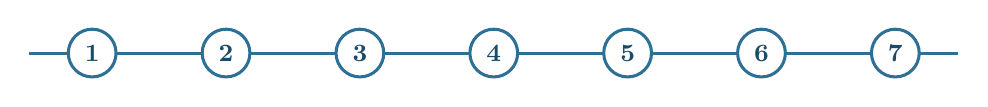
\begin{tikzpicture}[baseline=0pt]
    \draw[accent, line width=1.1pt] (0.9,0) -- (12.7,0);
    \foreach \i in {1,...,7} {
      \node[draw=accent, fill=white, circle, minimum size=17pt, line width=1.1pt,
            font=\fontsize{9}{9}\selectfont\bfseries, text=accentdark] at (\i*1.7,0) {\i};
    }
  \end{tikzpicture}
  \end{center}
  \vspace{-6pt}
  \noindent{\footnotesize\itshape\color{accentdark} #2\hfill #3}\\[3pt]
}

% --- Fill-in-the-blank field: label + underline ------------------------------
\newcommand{\blank}[2]{{\footnotesize\color{accentdark}#1}: \makebox[#2]{\hrulefill}}

\begin{document}

\noindent\colorbox{accent}{\parbox{\dimexpr\linewidth-2\fboxsep}{%
  \centering\color{white}%
  {\bfseries\LARGE Post-Trial Questionnaire}\\[3pt]
  {\footnotesize Complete once per condition, after both worlds have been tried under it.}%
}}
\\[10pt]

\noindent\colorbox{accentlight}{\parbox{\dimexpr\linewidth-2\fboxsep}{%
  \blank{Participant}{2.4cm}\hfill\blank{Condition (e.g.\ JFB)}{2.2cm}\hfill\blank{Date}{3.0cm}%
}}
\\[8pt]

{\footnotesize\itshape\color{accentdark} Circle one number per scale, 1--7, unless noted otherwise. There are no right answers -- answer how the condition actually felt overall.\par}

\sectionbar{A. Workload (NASA Task Load Index\footnote{\footnotesize Hart \& Staveland (1988), \textit{NASA-TLX}; trimmed to 3 subscales and adapted to a 7-point scale.})}

\scaleseven{1. Mental Demand -- How mentally demanding was the task?}{Very Low}{Very High}
\scaleseven{2. Physical Demand -- How physically demanding was the task?}{Very Low}{Very High}
\scaleseven{3. Performance -- How successful were you in accomplishing the task?}{Perfect}{Failure}

\sectionbar{B. Control, Trust \& Comfort\footnote{\footnotesize Items adapted from standard HRI trust/control constructs, e.g.\ Jian, Bisantz \& Drury (2000).}}

\scaleseven{4. I felt in control of the robot's motion.}{Strongly Disagree}{Strongly Agree}
\scaleseven{5. I trusted the robot to do what I intended.}{Strongly Disagree}{Strongly Agree}
\scaleseven{6. The robot's motion felt smooth and comfortable.}{Strongly Disagree}{Strongly Agree}

\sectionbar{C. Notes}
{\footnotesize\itshape\color{accentdark} Anything notable about this condition? (optional)\par}
\vspace{6pt}
\textcolor{accent}{\rule{\linewidth}{0.6pt}}\\[9pt]
\textcolor{accent}{\rule{\linewidth}{0.6pt}}\\[9pt]
\textcolor{accent}{\rule{\linewidth}{0.6pt}}\\[9pt]
\textcolor{accent}{\rule{\linewidth}{0.6pt}}

\end{document}
